\documentclass{article}

% preambulo:
\usepackage[utf8]{inputenc}
% caracteres utf8 (tildes, enie) sin tener que usar comandos

\usepackage[spanish, es-tabla, es-nodecimaldot]{babel} 
% texto automatico en espaniol
% "tabla" en vez de "cuadro"
% no reemplaza puntos decimales por comas

%% NO AGREGAR PAQUETES ANTES DE ESTO, ES IMPORTANTE QUE BABEL ESTE PRIMERO

%%%%%%%%%%%%%%%%%%%%%%%%%%%%%%%%%
%% PAQUETES EXTRA %%%%%%%%%%%%%%%
%%%%%%%%%%%%%%%%%%%%%%%%%%%%%%%%%

\usepackage{subfiles}

%nuevo
\usepackage[notransparent]{svg}
%

\usepackage{amsmath} % PAQUETES DE MATEMATICA
\usepackage{amsfonts}
\usepackage{amssymb}

%puse esta cosa nueva---
\usepackage{csvsimple}

%-----
\usepackage{steinmetz} % comando \phase{}
\usepackage{units} % permite usar nicefrac
\usepackage{graphicx} % importar imagenes
\usepackage{float} % posicion H para floats
\usepackage[colorinlistoftodos]{todonotes}


\usepackage[a4paper, total={6in, 8in}]{geometry} 
% margenes correctos en subarchivos

\setlength{\parindent}{10pt}			%cuanta sangria al principio de un parrafo
\usepackage{indentfirst}				%pone sangria al primer parrafo de una seccion

\usepackage{listings}

\usepackage{color}

\definecolor{codegreen}{rgb}{0,0.6,0}
\definecolor{codegray}{rgb}{0.5,0.5,0.5}
\definecolor{codepurple}{rgb}{0.58,0,0.82}
\definecolor{backcolour}{rgb}{0.95,0.95,0.92}
 
\lstdefinestyle{mystyle}{
    backgroundcolor=\color{backcolour},   
    commentstyle=\color{codegreen},
    keywordstyle=\color{magenta},
    numberstyle=\tiny\color{codegray},
    stringstyle=\color{codepurple},
    basicstyle=\footnotesize,
    breakatwhitespace=false,         
    breaklines=true,                 
    captionpos=b,                    
    keepspaces=true,                 
    numbers=left,                    
    numbersep=5pt,                  
    showspaces=false,                
    showstringspaces=false,
    showtabs=false,                  
    tabsize=2
}
 
\lstset{style=mystyle}

%%%%%%%%%%%%%%%%%%%%%%%%%%%%%%%%%%%%%%%%%%%%%%%%%%%%%%%%%%%
%% NO AGREGAR PAQUETES DESPUES DE ESTO, ES IMPORTANTE QUE HYPERREF ESTE ULTIMO
\usepackage[hidelinks]{hyperref} % hipervinculos sin cajitas rojas
\usepackage{bm}


\usepackage{fancyhdr}

\geometry{top=2.5cm, bottom=2.0cm, left=2.25cm, right=2.25cm}

\lhead{Sistemas de Control 22.85}
\chead{TP3 - Control Servo}
\rhead{ITBA}
\renewcommand{\headrulewidth}{1pt}
\renewcommand{\footrulewidth}{1pt}
\pagestyle{fancy}


\begin{document}

%\newgeometry{} % margenes default para la caratula
% caratula:
\begin{titlepage}
\newcommand{\HRule}{\rule{\linewidth}{0.5mm}}
\center
\mbox{\textsc{\LARGE \bfseries {Instituto Tecnol\'ogico de Buenos Aires}}}\\[1.5cm]
\textsc{\Large 22.85 - Sistemas de Control}\\[0.5cm]


\HRule \\[0.6cm]
{ \Huge \bfseries Trabajo de Laboratorio N$^{\circ}$3: Control Servo por Realimentación lineal de Estados}\\[0.4cm] % Title of your document
\HRule \\[1.5cm]


{\large

\emph{Grupo 2}\\
\vspace{3px}

\begin{tabular}{lr} 	
\textsc{M\'aspero}, Martina  & 57120 \\
\textsc{Mestanza}, Joaqu\'in Mat\'ias  & 58288 \\
\textsc{Nowik}, Ariel Santiago  & 58309 \\
\textsc{Panaggio Venerandi}, Guido Martin  & 56214 \\
\textsc{Parra}, Roc\'io  & 57669 \\
\textsc{Regueira}, Marcelo Daniel  & 58300 \\

\end{tabular}

\vspace{20px}

\emph{Profesor}\\
\vspace{3px}
\textsc{Nasini}, V\'ictor Gustavo\\ 	
\vspace{100px}

\begin{tabular}{ll}

Presentado: & 13/11/2019\\

\end{tabular}

}

\vfill

\end{titlepage}


% indice:
\tableofcontents
\newpage

\section{Análisis del Motor de CC}

En primer lugar se considera el modelo circuital para el motor utilizado, teniendo en cuenta que los diferentes parámetros son datos provistos por la hoja de datos del QUANSER:

\begin{figure}[H]
\centering
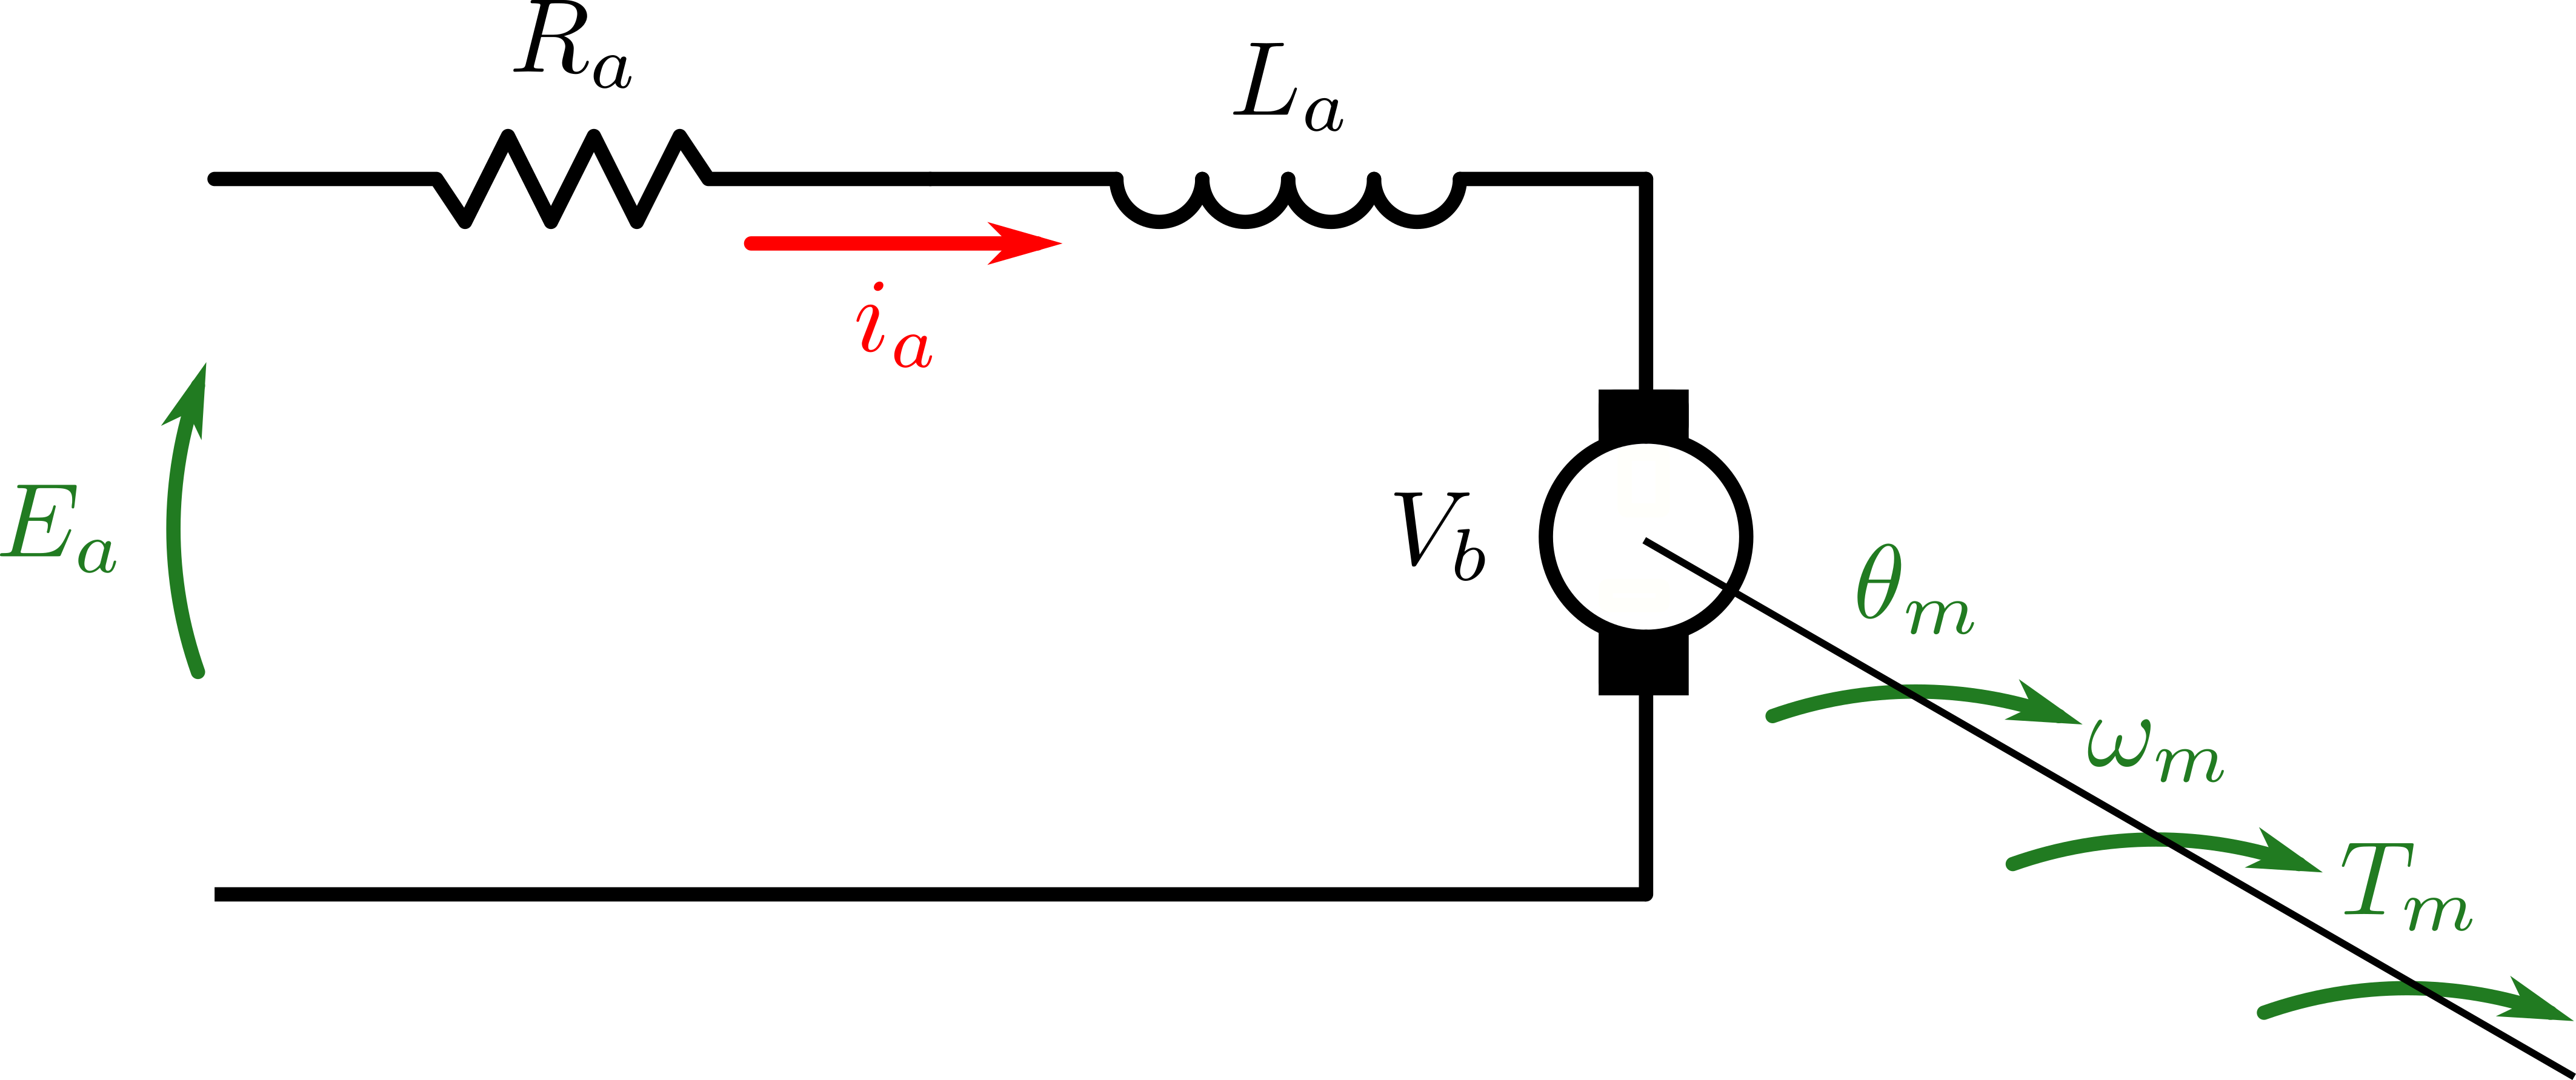
\includegraphics[width=0.5\linewidth]{../Images/ModeloMotor.png}
\end{figure}

Las ecuaciones que caracterizan al sistema son:

\[
\left\lbrace
\begin{array}{ll}
E_a = R_a \cdot i_a + L_a \cdot \dot{i_a} + V_b \\
V_b = K_b \cdot \omega_m = K_b \cdot \dot{\theta_m} \\
T_m = J_m \cdot \ddot{\theta_m} + B_m \cdot \dot{\theta_m} + T_l
\end{array}
\right.
\]

De las cuales se puede obtener las funciones de transferencia de $\theta_l$ y $\omega_m$ respecto a la tensión de alimentación $E_a$:

\[
\frac{\omega_m}{E_a} = \frac{\frac{K_t}{R_a \cdot J_m}}{S + \frac{B_m}{J_m} + \frac{K_t \cdot K_b}{R_a \cdot J_m}}
\]

\[
\frac{\theta_m}{E_a} = \frac{\frac{K_t}{R_a \cdot J_m}}{S \cdot (S + \frac{B_m}{J_m} + \frac{K_t \cdot K_b}{R_a \cdot J_m})}
\]

\end{document}
